\documentclass[11pt]{article}
\usepackage[margin=1in]{geometry}
\usepackage{amsmath,amssymb}
\usepackage{graphicx}
\usepackage[hidelinks]{hyperref}

\newcommand{\arxiv}[1]{\href{https://arxiv.org/abs/#1}{arXiv:#1}}
\newcommand{\weakfpp}{weak-FPP}

\title{Literature-Implied Partial Answer: Weak-FPP Under A Block-Basis Hypothesis}
\author{FA/Banach run \texttt{fa\_banach\_001}}
\date{2026-06-14}

\begin{document}
\maketitle

\section*{Status}

This packet records a \emph{literature-implied partial subcase}, not an
original proof and not a full solution of the unconditional-basis
\weakfpp{} problem.  Barroso \arxiv{2012.10849} states that it remains open
whether every Banach space with an unconditional basis has the weak fixed
point property.  Barroso's later paper \arxiv{2302.11287} proves an
affirmative result for a structurally restricted subcase: bases whose block
basis sequences always contain a subsequence equivalent to the original basis.

\section*{Original Question}

The original source is:
\begin{quote}
C. S. Barroso, \emph{Isometric embeddings of Banach spaces under optimal
projection constants}, \arxiv{2012.10849}.
\end{quote}

In the metric fixed point application section, after recalling Lin's theorem,
the paper says that it is still open whether every Banach space with an
unconditional basis has the \weakfpp{}.

\begin{center}

\includegraphics[width=0.96\linewidth]{figures/open_problem_crop.png}
\end{center}

The same source paper proves a shrinking \(D\)-unconditional subcase with
\(D<\sqrt{6}-1\).  That same-paper result is treated only as context here, not
as a packet-worthy literature answer.

\section*{Supporting Literature}

The supporting source is:
\begin{quote}
C. S. Barroso, \emph{Remarks on the FPP in Banach spaces with unconditional
Schauder basis}, \arxiv{2302.11287}.
\end{quote}

The later paper explicitly formulates the broad unconditional-basis question
and the \(1\)-suppression unconditional version:

\begin{center}
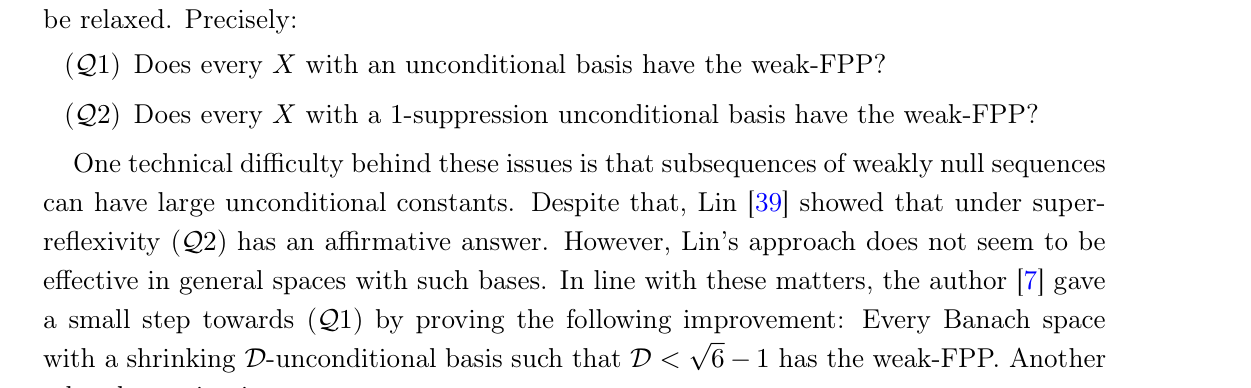
\includegraphics[width=0.96\linewidth]{figures/supporting_context_crop.png}
\end{center}

Its Theorem 3.11 states:

\begin{center}

\includegraphics[width=0.96\linewidth]{figures/supporting_theorem_crop.png}
\end{center}

\section*{Proof Intuition}

The later theorem supplies the missing fixed point conclusion directly once
the original question is narrowed by a strong block-basis regularity
hypothesis.  The branch in which the given basis is \(1\)-suppression
unconditional is a subcase of having an unconditional basis.  The additional
assumption, that every block basis sequence contains a subsequence equivalent
to the original basis, is the structural ingredient that lets the supporting
paper run its spreading-model and weakly-null sequence argument.

\section*{Theorem Recorded}

\textbf{Claim.}
Let \(X\) be a Banach space with a Schauder basis \((e_i)\).  Suppose:
\begin{enumerate}
\item \((e_i)\) is \(1\)-suppression unconditional; and
\item every block basis sequence of \((e_i)\) has a subsequence equivalent to
  \((e_i)\).
\end{enumerate}
Then \(X\) has the weak fixed point property.

\section*{Proof}

This is exactly the \(1\)-suppression unconditional branch of Theorem 3.11 in
Barroso \arxiv{2302.11287}.  The theorem assumes that \(X\) has a Schauder
basis \((e_i)\) such that every block basis sequence has a subsequence
equivalent to the basis.  It then concludes that \(X\) has the weak fixed
point property in each of two cases, the first being that \((e_i)\) is a
\(1\)-suppression unconditional basis.  These are precisely the two
hypotheses listed above, so the conclusion follows.

Because a \(1\)-suppression unconditional basis is unconditional, this gives
an affirmative answer to the original unconditional-basis question for this
restricted class of spaces.

\section*{Scope And Limitations}

\begin{itemize}
\item The full question ``Does every Banach space with an unconditional basis
  have the weak-FPP?'' remains open in the sources checked here.
\item The packet does not answer the question for all \(1\)-suppression
  unconditional bases; the block-basis-equivalence hypothesis is part of the
  result.
\item Theorem 3.11 also covers a \(1\)-spreading-basis branch.  This packet
  does not use that branch as the main match, because the direct subcase of
  the original unconditional-basis problem is the \(1\)-suppression
  unconditional branch.
\item The packet records a direct literature implication from
  \arxiv{2302.11287}; it is not a new proof from this run.
\end{itemize}

\section*{Verification Notes}

The source statement was checked in \arxiv{2012.10849}, page 5.  The
supporting theorem was checked in \arxiv{2302.11287}, page 8.  A bounded web
search on 2026-06-14 for exact phrases around ``every Banach space with an
unconditional basis'' and ``weak fixed point property'' found the same 2023
follow-up paper and did not show a later full resolution of the broad
question.  The later paper itself phrases the broad questions \((Q1)\) and
\((Q2)\), cites the 2020 paper as a small step, and provides the restricted
Theorem 3.11 recorded above.

No computational verification is relevant.

\section*{Human Review Recommendation}

Keep the classification as \emph{literature-implied partial subcase}.  The
main reviewer check is that the block-basis assumption in Theorem 3.11 has
not been accidentally omitted when comparing to the original open question.

\begin{thebibliography}{9}

\bibitem{Barroso2020}
C. S. Barroso,
\emph{Isometric embeddings of Banach spaces under optimal projection
constants},
\arxiv{2012.10849}.

\bibitem{Barroso2023}
C. S. Barroso,
\emph{Remarks on the FPP in Banach spaces with unconditional Schauder basis},
\arxiv{2302.11287}.

\end{thebibliography}

\end{document}
